\documentclass[journal=jacsat,manuscript=article]{achemso}
\usepackage{paper_style}

%\usepackage{lipsum}  %% Package to create dummy text (comment or erase before start)

%% ===============================================
%% Setting the line spacing (3 options: only pick one)
\doublespacing
% \singlespacing
%\onehalfspacing
%% ===============================================


% %%%%%%%%%%%%%%%%%%%%%%%%%%%%%%%%%%%%%%%%%%%%%%%%%%%%%%%%%%
% SET THE TITLE
% %%%%%%%%%%%%%%%%%%%%%%%%%%%%%%%%%%%%%%%%%%%%%%%%%%%%%%%%%%

% TITLE:
\title{
First-Principles Studies of Substituent Effect on Squaraine Dyes\\
}

% AUTHORS:
\author{German Barcenas}
\affiliation{Boise State University}
\email{germanbarcenas@u.boisestate.edu}
\author{Austin Biaggne}
\affiliation{Boise State University}
\author{Kimo Wilson}
\affiliation{Boise State University}
\author{Bill Knowlton}
\affiliation{Boise State University}
\author{Bernard Yurke}
\affiliation{Boise State University}
\author{Lan Li}
\affiliation{Boise State University}





\begin{document}

\maketitle
% %%%%%%%%%%%%%%%%%%%%%%%%%%%%%%%%%%%%%%%%%%%%%%%%%%%%%%%%%%
% %%%%%%%%%%%%%%%%%%%%%%%%%%%%%%%%%%%%%%%%%%%%%%%%%%%%%%%%%%
% BODY OF THE DOCUMENT
% %%%%%%%%%%%%%%%%%%%%%%%%%%%%%%%%%%%%%%%%%%%%%%%%%%%%%%%%%%
% %%%%%%%%%%%%%%%%%%%%%%%%%%%%%%%%%%%%%%%%%%%%%%%%%%%%%%%%%%

% --------------------
\section{Introduction}
% --------------------
Employing DNA self-assembly methods is shown to enable the manipulation and mediation of chromophore dyes and give rise to Frenkel exciton delocalization among dimer systems\cite{Cannon2018LargeAggregates}. The study of monomers can lend insight into suitable candidates for more highly tuned dimer systems. Squaraine dyes in particular are reported to have spectral properties that make them a strong candidate to be used in conjunction with DNA nanotechnology\cite{Markova2013ComparisonLabels}⁠. This application of squaraines offers an opportunity to implement multichromophoric systems. 
By utilizing DNA as a scaffold for squaraiane aggregation, dipole-dipole coupling occurs\cite{Cannon2017CoherentSystem}. This interatomic interaction model was first described by Kasha to allow the mixing of wavefunctions to access nondegenerate states\cite{Kasha1965TheSpectroscopy}. The splitting of energy levels results in new excited state behavior in aggregates as a bathochromic shift in absorbance (often referred as an J aggregate) or a hypsochromic shift (often referred to as an H aggregate) in conjunction with an observed splitting of the absorption peak known as Davydov splitting\cite{Zhong2019DavydovDimers}. The optical properties of these aggregates results in Frenkel excitons with coupling strengths related to these newly accessible states. 
It is important to begin the study of a dye monomer to establish a baseline of to multicomponent systems. Although aggregates are defined by their interaction distances, monomer electronic information is necessary when treating these interactions with point dipole approximations\cite{Abramavicius2009ExtractingSpectra}. Examples of other fields in which squaraines are being applied include organic photovoltaics\citep{Wei2012FunctionalizedPhotovoltaics, Chen2018DensityCell}, near infrared medical imaging\cite{Strassel2018SquaraineNm}⁠, and molecular photoswitches\citep{Kellis2019AnPhases, Scholes2011LessonsHarvesting} .

Squaraine dyes are composed of a squaric acid center. This central feature is a made from a electron-deficient aromatic group. This group is then combined with accepting of electron-rich groups, often in a symmetric manner by means of a methine bridge\cite{Ilina2020SquaraineChallenges}⁠. In this study, the electron-rich groups are trimethylindolenine with varied substitutes.

Previous work\cite{Bassal2017ExploringADC2}⁠ highlights the history of computational studies of squaraine dye studies. This work presents a smaller variation in squaraine dyes by maintaining the basic chemistry and only altering substituent groups. Squaraine dyes, unlike similar NIR cyanine dyes, are not symmetric and so from the monomer perspective have a potential for conformers to influence bulk spectral properties\cite{Kolosova2018MolecularSquaraines}⁠. Highlighting squaraine conformer properties has recently become of interest due to the conformations potential to alter the final photophysical properties in squaraine applications\cite{Paterno2018ExcitedScenario}⁠.  Conformers investigated in this paper are : trans,syn; cis,syn; and trans,anti.

This work investigates the ground state and excited state molecular structure of three conformations: trans,syn; cis,syn, and trans,anti for SQ1--SQ(i)-H2,SQ4--SQ(i)-Cl2 ,SQ8--SQ(i)-Cl1 and SQ14--SQ(i)-(CH3)2 otherwise referred to as SQ1, SQ4, SQ8 and SQ14 using density functional theory. This work presents a study of SQ1, SQ4, SQ8, and SQ14, in which substituents are changed according to their name. Investigations into the ground state and excited state electronic structures of these chromophores will enable a comparison of different substituents and their effects on electronic transition states necessary for the optimization of multichromophoric systems while also considering absorption properties. Cyanine dyes have also been known to exhibit similar behavior and offer another opportunity for comparison\cite{Fothergill2018AbDyes}.


% --------------------
\section{Methodology}
% --------------------
Gaussian 16 software package\cite{M.J.FrischG.W.Trucks2016Gaussian09}⁠ was used in density functional density calculations. Molecules were built and initially relaxed using the molecular editing software Avogadro\cite{Hanwell2012Avogadro:Platform}⁠ using the UFF\cite{Rappe1992UFFSimulations}⁠ method. All calculations were performed using the 6-31G+(d,p) basis set with the M06-2X\cite{Zhao2008TheFunction}⁠ correlation functional as previous works have shown a strong agreement with experimental results when compared with physical systems\cite{Jacquemin2016Excited-StateCC2}. These structures were optimized using a tight root mean square residual force of $1*(10)^{-5}$  Hartree$⁄$Bohr and an ultra fine integration grid of $99$ radial shells and $590$ angular points per shell. The use of tight root mean squared and ultra fine integration grid is recommended for optimizing larger molecules with soft frequency modes such as methyl groups\cite{AzaisTestingSuper-Resolution}⁠ . Ground state optimization of these molecules were verified to be optimized via ground state frequency checks to ensure no imaginary frequencies were present. The optimized ground state structures were then used as the input geometry for excited state optimization calculations. The calculated excited state geometry was used to calculate the excited state frequency to ensure an optimized structure was achieved.  The ground state and excited state frequencies were then used to produce an absorption spectrum for each molecule and conformer. These spectra were generated using the general Frank-Condon (FC) method. 

Conformation of squaraine dyes are referred here as trans,syn; cis,syn and trans,anti. In the study of monomers, it has been reported that there is a potential for coexistence of conformers in solution\cite{Kolosova2019MolecularSquaraines}⁠. The population percentages were investigated to using the Boltzmann distribution. 

$\Del$E$_{0-0$ vs $\Del$E$_{?}$ 
Experimental discussion? Talk to Kimo

\section{Results}
When comparing the results of conformer to experimental conditions and Boltzmann population distributions, the trans,anti conformation is the most dominate population and is closest to the experimental peak absorbance. This is in agreement with previous work by Kolosova et al. All spectrum exhibit a weak vibronic shoulder followed by a strong absorption in the orange wavelength region.

What is the expected absorption of trimethlyindole?


\begin{figure}[h]
    \centering
    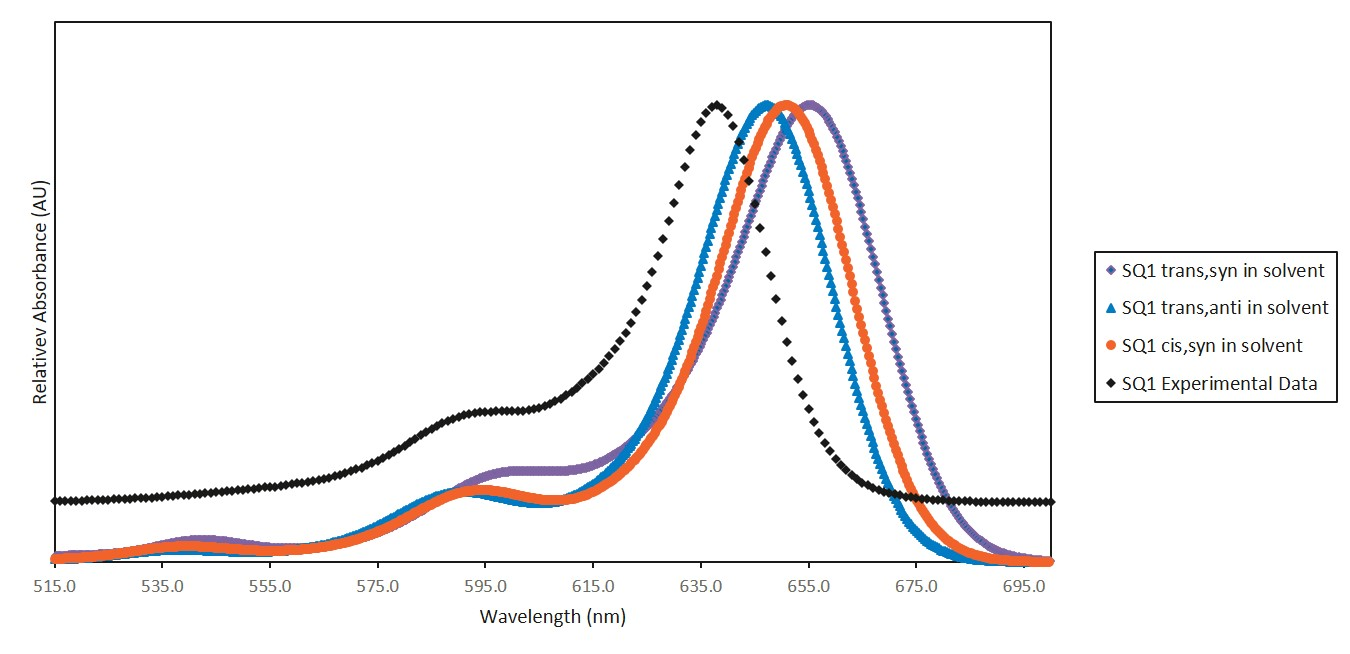
\includegraphics[width=16cm,height=8cm]{figures/sq1_conformer_exp.jpg}
    \caption{Comparison of SQ1—Sq(i)-H2 conformer spectra generated using FC approximation in IEFPCM water solvent. All structures were optimized  using 6-31+G(d,p) basis set and M06-2X exchange correlation functional.}
    \label{fig:SQ1 conformers}
\end{figure}

When comparing SQ1 and SQ4 trans,anti, experimental results, and vacuum calculations, we can see that M06-2X in vacuum is able to predict experimental absorption spectrum before the inclusion of a solvent. The inclusion of solvent is able to predict the peak within X$\%$ of experiment. The blue shift of X$\%$ is a well-known phenomena of TD-DFT calculations with this family of cyanine-type dyes. This shift is applied to all dyes an so there is still a shift from the Cl substiuents in SQ4.   
\begin{figure}[h]
    \centering
    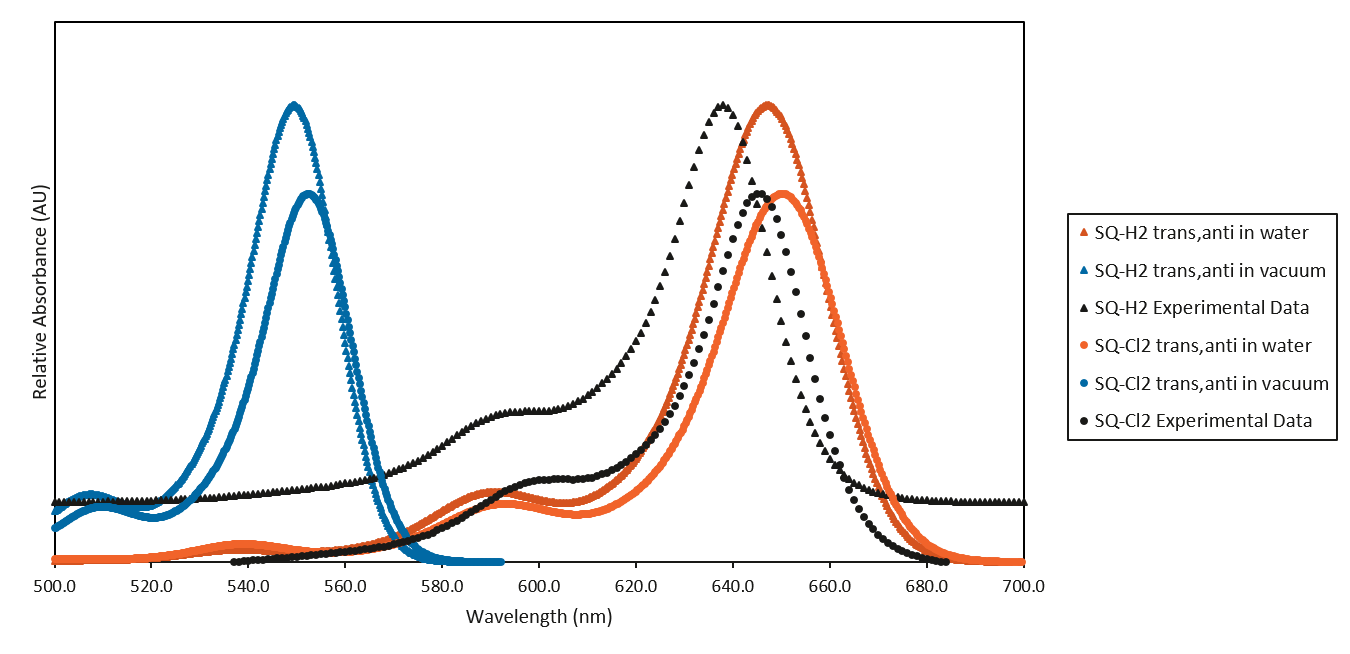
\includegraphics[width=15cm,height=8cm]{figures/sq1-sq4.png}
    \caption{Comparison of  SQ1—Sq(i)-H2 and SQ4—SQ(i)-Cl2 spectra generated using FC approximation in vacuum, IEFPCM water solvent, and experimental data. All structures were optimized using 6-31+G(d,p) basis set and M06-2X exchange correlation functional.}
    \label{fig:SQ1 and SQ4}
\end{figure}
\newpage

\newpage
\newpage
\begin{figure}[h]
    \centering
    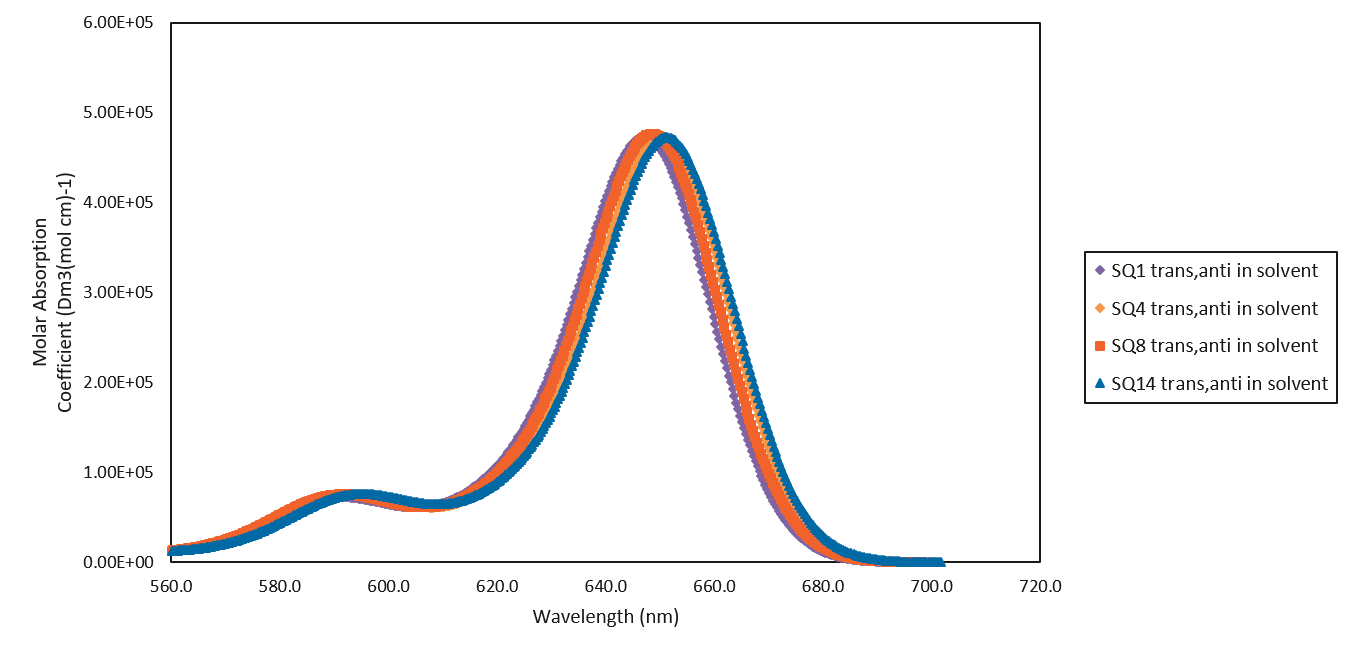
\includegraphics[width=15cm,height=8cm]{figures/sq1_4_8_14.png}
    \caption{Comparison of  SQ1—Sq(i)-H2, SQ4—SQ(i)-Cl2, SQ8—SQ8(i)-Cl1, and SQ14—SQ(i)-(CH3)2 trans,anti conformation spectra generated using FC approximation in IEFPCM water solvent. All structures were optimized  using 6-31+G(d,p) basis set and M06-2X exchange correlation functional.}
    \label{tab:SQ1,4,8,14 absorption}
\end{figure}

\newpage
\begin{table}[h]
    \centering
    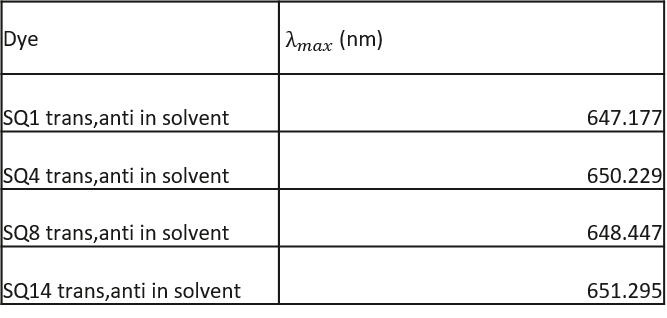
\includegraphics[width=8cm,height=4cm]{figures/sq1_4_8_14-table.png}
    \caption{SQ1-SQ(i)--H2, SQ4-SQ(i)--Cl2 ,SQ8--SQ(i)--Cl1, and SQ14-SQ(i)-(CH3)2 peak absorption data using FC approximation. All structures were optimized using 6-31+G(d,p) basis set and M06-2X exchange correlation functional in IEF-PCM water solvent.}
    \label{tab:SQ1,4,8,14 lambda data}
\end{table}
\begin{table}[h]
    \centering
    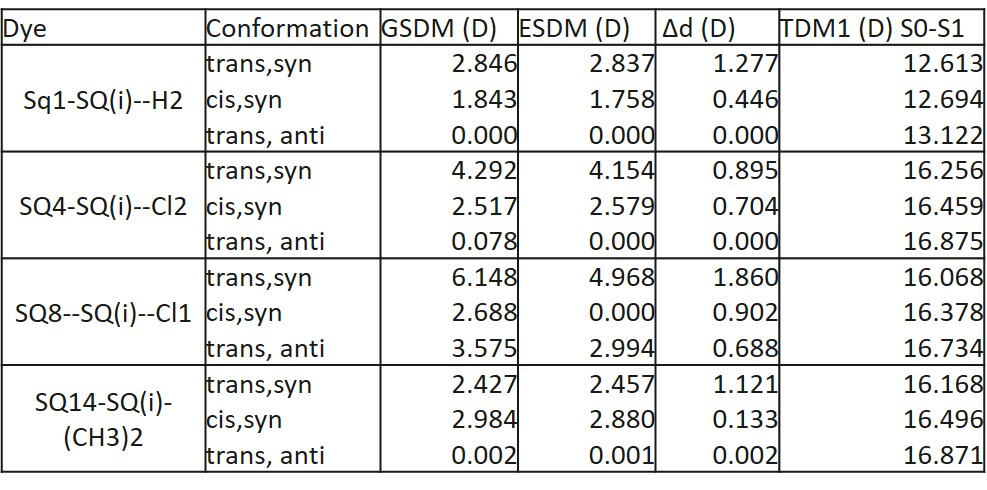
\includegraphics[width=13cm,height=6cm]{SQ1_4_8_14_electronic_table.jpg}
        \caption{SQ1-SQ(i)--H2, SQ4-SQ(i)--Cl2 ,SQ8--SQ(i)--Cl1, and SQ14-SQ(i)-(CH3)2 ground state dipole moment (GSDM), excited state dipole moment (ESDM), static difference dipole (Δd) and transition state dipole moment to the first excited state (TDM1). All structures were optimized using 6-31+G(d,p) basis set and M06-2X exchange correlation functional in IEF-PCM water solvent.}
    \label{tab:SQ1,4,8,14 electonic data}
\end{table}
\newpage
The altering of substituents of trimethylindolenine squaraine dyes does not significantly alter the peak absorption of these dyes. Meanwhile, these substituents allow for an opportunity to change the electronic properties of dyes. When comparing trans,anti data in Table \ref{tab:SQ1,4,8,14 electonic data}, the molecule with a break in symmetry, SQ8, exhibits a a difference dipole relative to the symmetric SQ1, SQ4, and SQ14. Meanwhile, when comparing the transition dipole of SQ4, SQ8, and SQ14, they remain relatively unperturbed. The difference between SQ4 and SQ14 in this case are none. When building a system meant for aggregation, these substituents can also effect the aggregation behavior. The inclusion of solution into the calculation can serve as a measure for likelihood of aggregation; more negative solvation energy is associated with a more thermdynamically favorable solution. For less negative solvation energy, the dyes  
\newpage
\newpage
\section{Conclusion}
Changing substituents allows for the changing of electronic properties while optical properties are help relatively constant. Trimethylindolenine squaraine dyes offer a the opportunity for highly tuned dye applications.
% %%%%%%%%%%%%%%%%%%%%%%%%%%%%%%%%%%%%%%%%%%%%%%%%%%%%%%%%%%
% %%%%%%%%%%%%%%%%%%%%%%%%%%%%%%%%%%%%%%%%%%%%%%%%%%%%%%%%%%
% REFERENCES SECTION
% %%%%%%%%%%%%%%%%%%%%%%%%%%%%%%%%%%%%%%%%%%%%%%%%%%%%%%%%%%
% %%%%%%%%%%%%%%%%%%%%%%%%%%%%%%%%%%%%%%%%%%%%%%%%%%%%%%%%%%

\newpage
\bibliography{references.bib} 

% ==========================
% ==========================
% ==========================


\end{document}